\begin{enumerate}[label=\thesection.\arabic*.,ref=\thesection.\theenumi]
\numberwithin{equation}{enumi}

\item An aircraft roll control system can be represented by a block diagram shown in  \ref{fig:ee18btech11048_block} with
\begin{align}
G\brak{s} &= \frac{10 K}{s\brak{s+1}\brak{s+5}}
\label{eq:ee18btech11048_system}
\end{align}

\begin{figure}[h]
 \centering
     \resizebox{\columnwidth}{!}{
\tikzstyle{block} = [draw, fill=white!20, rectangle, 
    minimum height=3em, minimum width=4em]
\tikzstyle{sum} = [draw, fill=white!20, circle, node distance=1cm]
\tikzstyle{input} = [coordinate]
\tikzstyle{output} = [coordinate]
\tikzstyle{pinstyle} = [pin edge={to-,thin,black}]
\begin{tikzpicture}[auto, node distance=2cm,>=latex']
    % We start by placing the blocks
    \node [input, name=input] {};
    \node [sum, right of=input,node distance=2cm] (sum) {$\sum_{}^{}$};
    \node [block, right of=sum] (controller) {$C(s)$};
    \node [block, right of=controller,
            node distance=2.5cm] (system) {G(s)};
    % We draw an edge between the controller and system block to 
    % calculate the coordinate u. We need it to place the measurement block. 
    \draw [->] (controller) -- node[name=u] {} (system);
    \node [output, right of=system] (output) {};
    \coordinate [below of=u] (tmp);

    % Once the nodes are placed, connecting them is easy. 
    \draw [draw,->] (input) -- node  {$X(s) $} (sum);
    \draw [->] (sum) -- node {$ $} (controller);
    \draw [->] (system) -- node [name=y] {$Y(s) $}(output);
    \draw [->] (input) -- node{$ $} node[pos=0.93]{$+$} (sum);
    \draw [->] (y) |- (tmp) -| node[pos=0.99] {$-$} 
        node [near end] {$ $} (sum);
    
\end{tikzpicture}
}
    \caption{}
    \label{fig:ee18btech11048_block}
\end{figure}
Design a lag compensator C\brak{s} for a 60$\degree $ phase margin and an appropriate error constant of 5.

\solution For unity feedback we have Velocity error constant $\brak{K_v}$

\begin{align}
K_v &= \lim_{s \to 0} s G\brak{s} 
\end{align}
\begin{align}
\lim_{s \to 0} \brak{\frac{10 K}{\brak{s+1}\brak{s+5}} }& = 5 \\
\implies K = 2.5
\end{align}
From Fig.\ref{fig: Graph 1}\\
Phase Margin  = 3.94\degree\\
Gain Crossover Frequency = 2.04 rad/s\\
\item 
\begin{figure}[!h]
\centering
  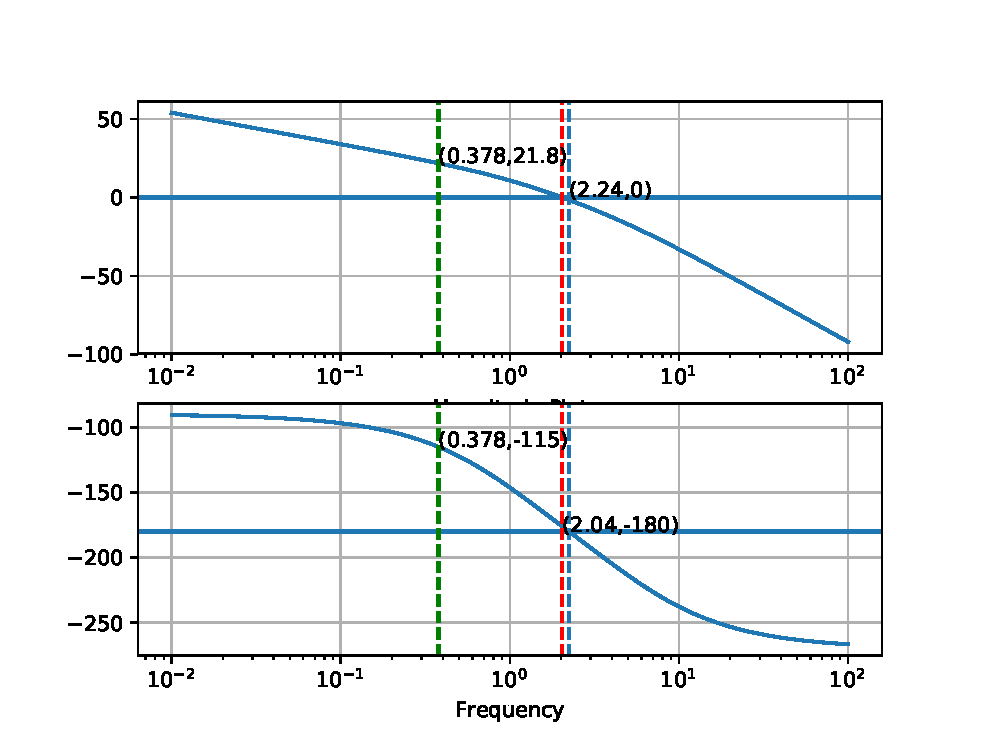
\includegraphics[width=\columnwidth]{./figs/ee18btech11048_1.eps}
  \caption{Graph 1}
  \label{fig: Graph 1}
\end{figure}

Finding Lag Compensator \brak{C\brak{s}} to yield a Phase margin of 60\degree \\
\solution 
\begin{align}
    C\brak{s} =& \frac{1}{\beta} \frac{\brak{s+\frac{1}{\tau}}}{\brak{s+\frac{1}{\tau\beta}}}
\end{align}
Phase Margin required = 60\degree
\begin{align}
\angle {C\brak{j\omega}} =& -180\degree+60\degree+5\degree \\
\angle {C\brak{j\omega}} =& -115\degree
\end{align}
For phase lag network 5\degree is added.\\
To obtain graph in Fig.\ref{fig: Graph 1} use the following code:
\begin{lstlisting}
codes/ee18btech11048_1.py
\end{lstlisting}

From Fig.\ref{fig: Graph 1}
\begin{align}
\angle {C\brak{j\omega}}=& -115\degree \\
\implies
\omega =& 0.37 rad/s\\
\implies
Gain =& 21.8dB\\
\end{align}
Calculating $\beta$ :
\begin{align}
-20log\frac{1}{\beta} =& 21.8\\
\implies \beta =& 12.3
\end{align}
Calculating $\frac{1}{\tau}$ :
\begin{align}
\frac{1}{\tau} =& \frac{0.37}{10}\\
\implies \frac{1}{\tau} =& 0.037
\end{align}

\begin{align}
C\brak{s} =& \frac{s+0.037}{12.3s+0.037}
\end{align}
\item 
Plotting the overall graph for C\brak{s}G\brak{s}.\\
Refer Fig \ref{fig: Graph 2}
\begin{align}
    C\brak{s}G\brak{s} &= \frac{s+0.037}{12.3s+0.037} \frac{25}{s\brak{s+1}\brak{s+5}}
\end{align}

\begin{figure}[!h]
\centering
  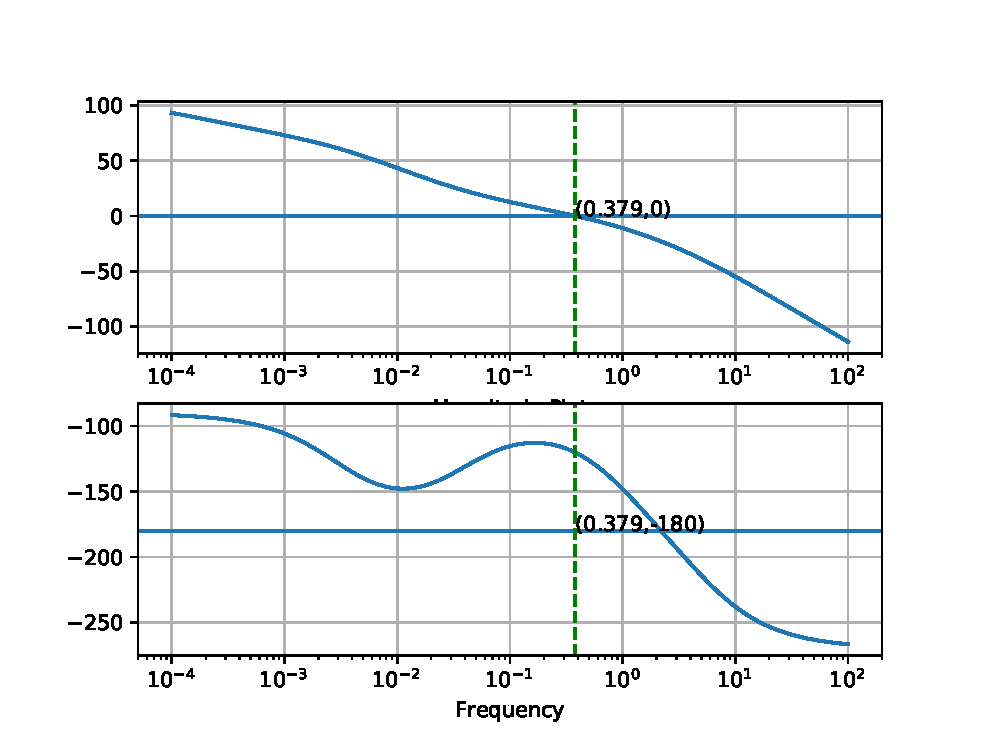
\includegraphics[width=\columnwidth]{./figs/ee18btech11048_2.eps}
  \caption{Graph 2}
  \label{fig: Graph 2}
\end{figure}
Phase Margin = 60\degree\\
To obtain graph in Fig.\ref{fig: Graph 2} use the following code:
\begin{lstlisting}
codes/ee18btech11048_2.py
\end{lstlisting}
\end{enumerate}
